\documentclass{article}

\usepackage[english]{babel}
\usepackage[utf8]{inputenc}
\usepackage{amsmath,amssymb}
\usepackage{parskip}
\usepackage{graphicx}
\usepackage{amsmath}
\usepackage{float}
\usepackage{url}

% Margins
%\usepackage[top=2cm, left=2.5cm, right=2.5cm, bottom=2.5cm]{geometry}
\usepackage[margin=1in]{geometry}
% Colour table cells
\usepackage{sectsty}
\usepackage{textcomp}
\usepackage{mathtools}
\usepackage[most]{tcolorbox}

% Get larger line spacing in table
%\newcommand{\tablespace}{\\[1.25mm]}
%newcommand\Tstrut{\rule{0pt}{2.6ex}}         % = `top' strut
%\newcommand\tstrut{\rule{0pt}{2.0ex}}         % = `top' strut
%\newcommand\Bstrut{\rule[-0.9ex]{0pt}{0pt}}   % = `bottom' strut

\sectionfont{\fontsize{12}{15}\selectfont}

%%%%%%%%%%%%%%%%%
%     Title     %
%%%%%%%%%%%%%%%%%
\title{Information Visualization - Project\vspace{-0.8em}}
\author{Marian Aldescu - MoSIG DS}
\date{\today}



\begin{document}
\maketitle



\textbf{\Large{Implement visualizations}}\\


\large{\textbf{Question: Which person, house, region, rank, title, institution pollutes the most?}}

\section{Initial vs actual design }
I will start by recalling the initial design of the visualization, which can be seen in Image \ref{fig:subsets}. The D3 implementation does not have major differences in terms of appearance: I kept the same position for each one of the 6 small plots, and also the structure of bar chart. A change that I did, which is not necessarily prominent, but it worth mentioning, is the modification of the bars orientation in the second row from horizontal to vertical: I consider it is important that their variation in height to match the orientation of the above 2 graphs. Also, the bars for the CO$_2$ emission over houses will vary now in height and not in width, as planned. The main reason is the large number of houses, I think a variation on the vertical axis would be clearer, than on the horizontal.

\begin{figure}[H]
	\centering
	\tcbox{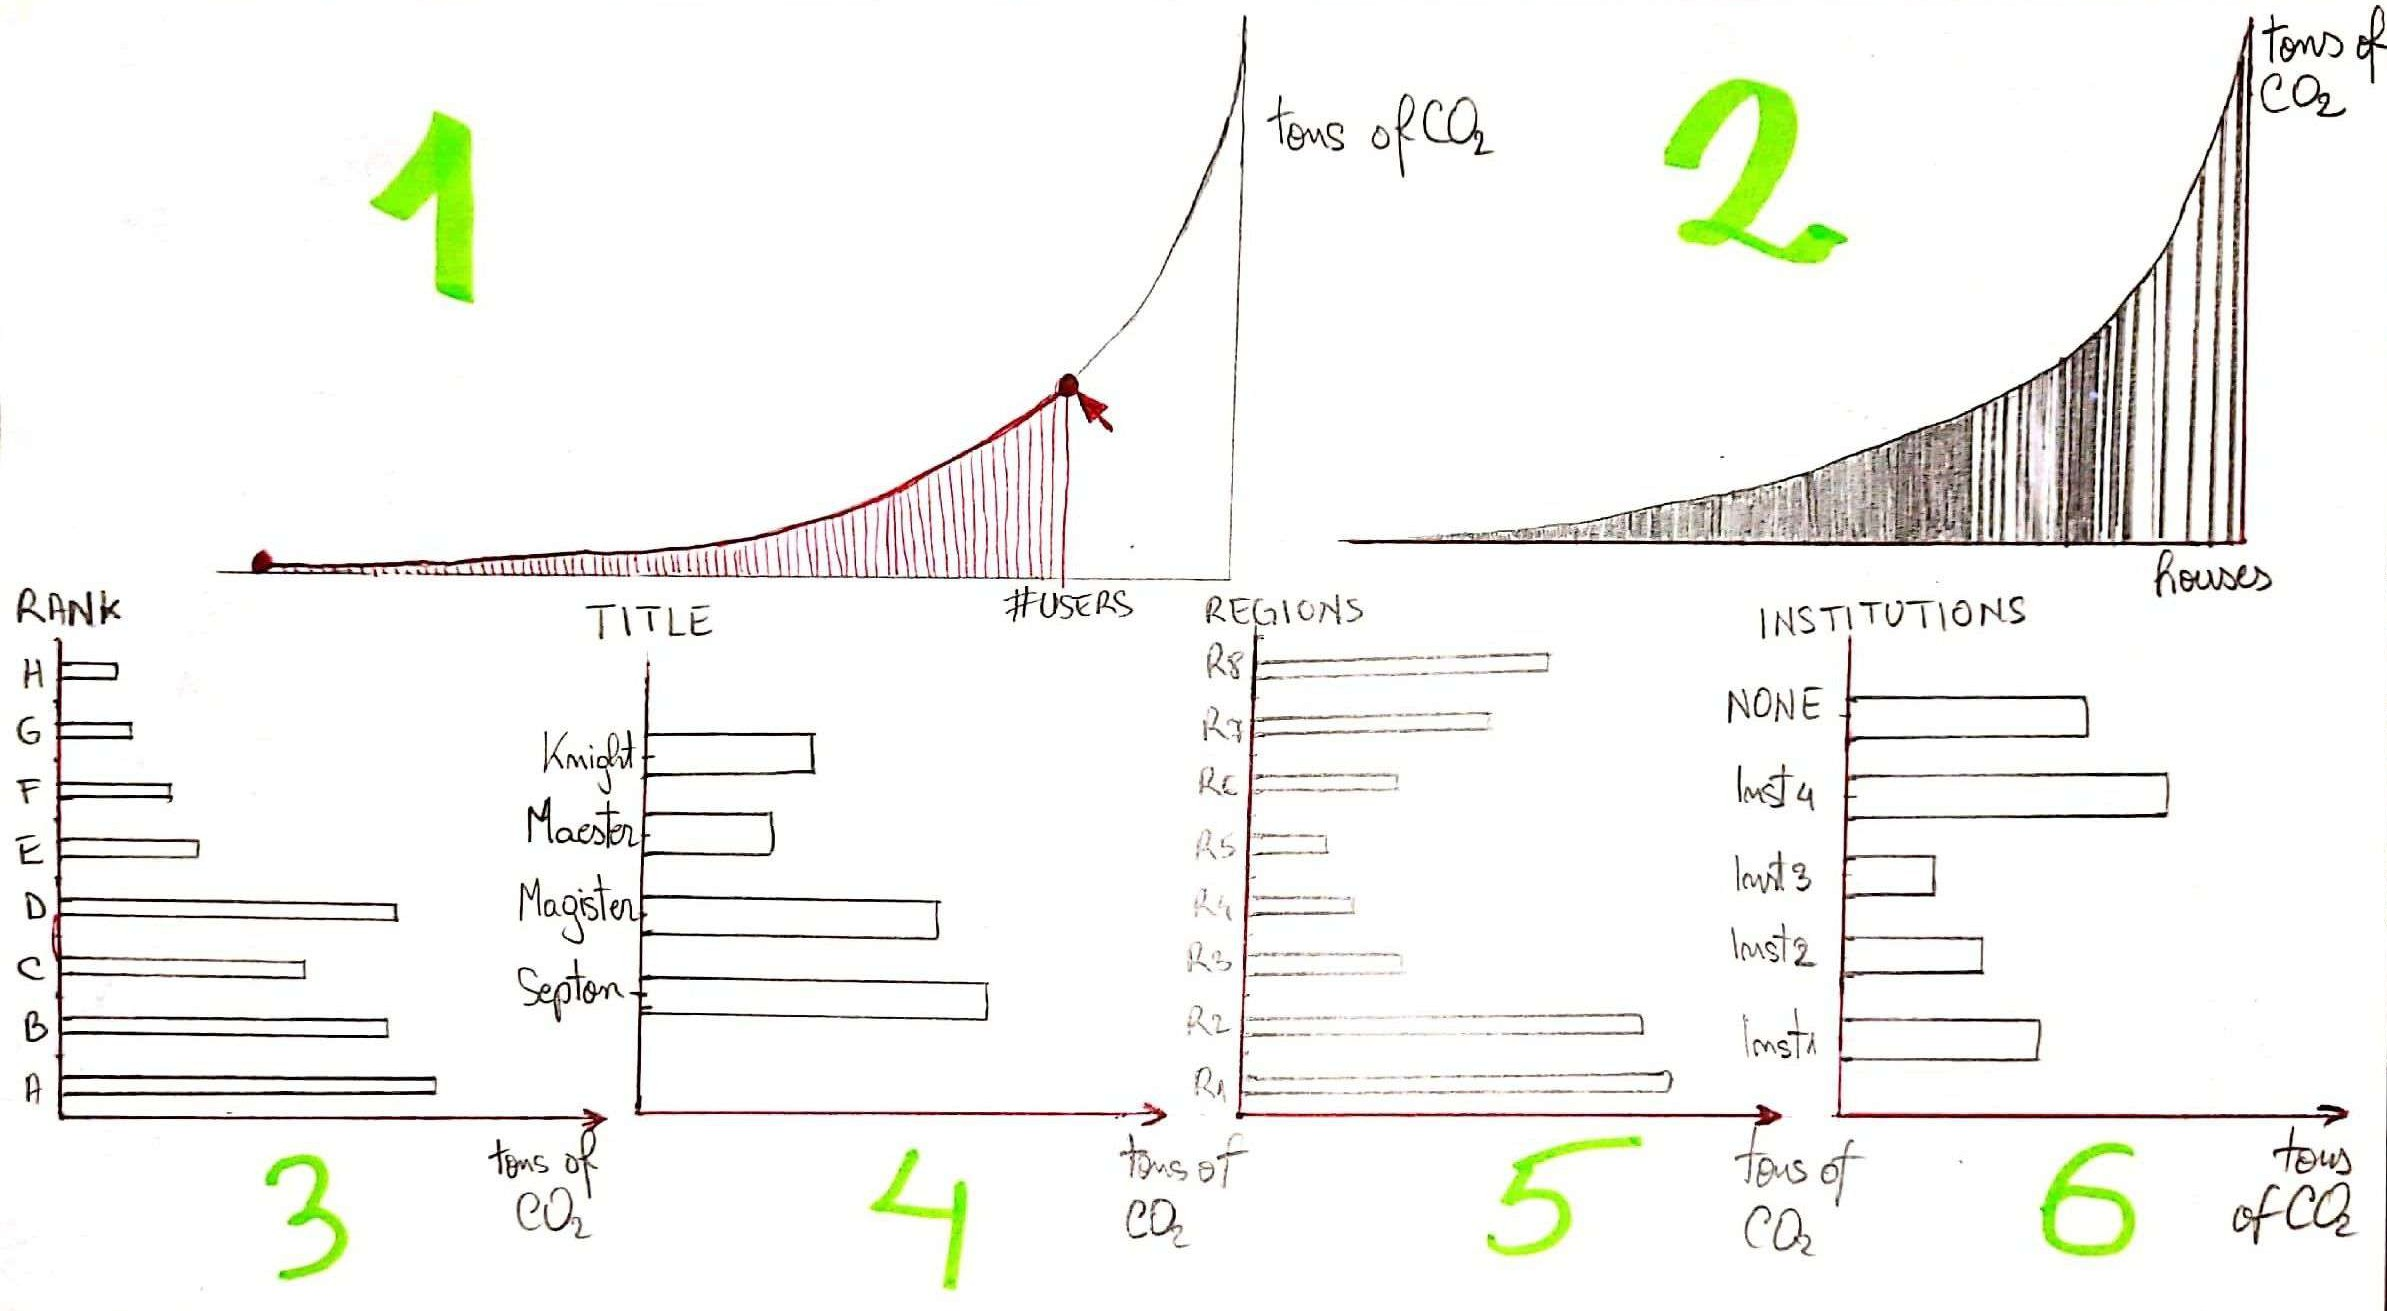
\includegraphics[scale=0.17]{img/8_5.jpg}}
	\caption{CO${_2}$ - subsets statistics(initial design)}
	\label{fig:subsets}
\end{figure}

\large{\textbf{Interaction trade-off}}\\

Initially, I intended to use a slider on the users CDF, in order to allow the examination of smaller groups. For this step, I found 2 libraries that allow filtering the subsets, more specifically: Crossfilter\cite{crossfilter} and DC\cite{dc}. I struggled to work with them, but due to the lack of time, I decided to make a compromise and choose a more "rigid" interaction, but that in the end could actually work. I split the first small plot in 6 equal vertical regions that are sensitive to mouse-over and click. By hovering the mouse above a region, this will change the color to differentiate it from the adjacent regions, and by clicking, the users of that region will be added to the other smaller plots. If a region is colored in blue, this is taken into consideration, if it is white, not. 


In Figure \ref{fig:vis_1} we can see an example in which all the dataset is analyzed.

\begin{figure}[H]
	\centering
	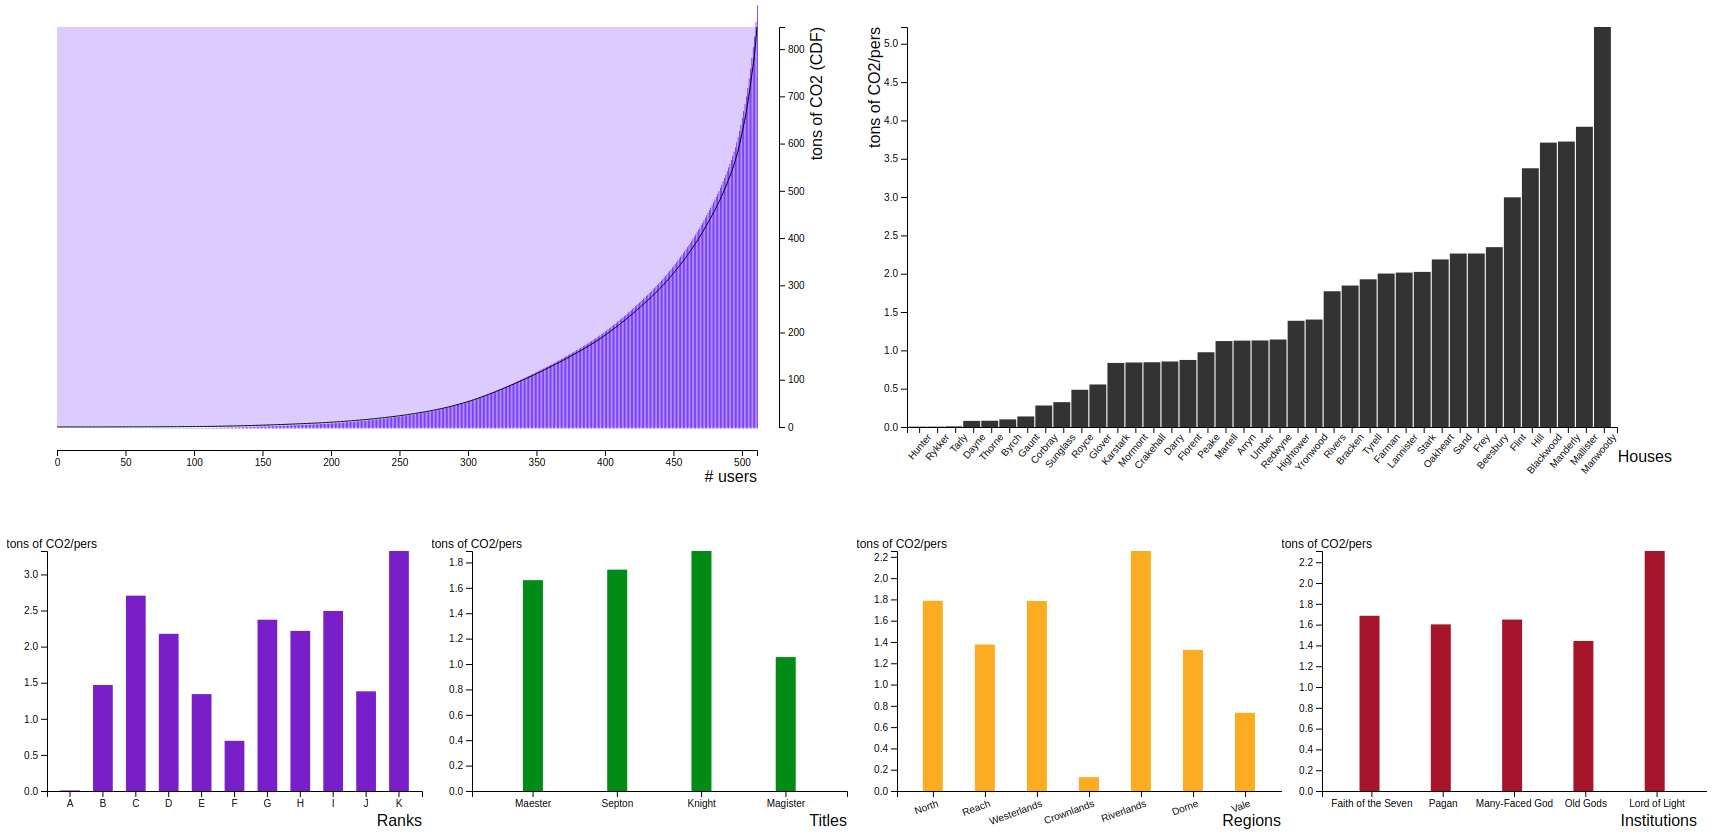
\includegraphics[scale=0.28]{img/ceo2.png}
	\caption{CO${_2}$ - subsets statistics. All users selected}
	\label{fig:vis_1}
\end{figure}

\section{From overview to details}

Before starting to discuss, note that the CO$_2$ emissions inside each house, rank title, region and institution are averaged by the number of users from that specific subset, because we do not want the size of the subsets to affect the perception. Therefore, the CO$_2$ level is expressed as an average of CO$_2$ tons/user.

When first looking at the visualization, we notice the almost exponential curve of the CDF chart. It is obvious that some users are polluting a lot more than others. Then, we notice that the houses CO$_2$ emissions fit almost the same distribution: the most pollutant houses can be seen in the right side(e.g. Manwoody, Mallister), on the other hand, the most "green" houses(e.g. Hunter, Rykker) seem to emit negligible quantities of CO$_2$. \\
Going to the second row of plots, we can easily see that some ranks produce very low CO$_2$ emissions(e.g. rank A), and they are very likely to live in the Crownlands region. Differences of the CO$_2$ emissions can be noticed also in the Titles(e.g. on average, users with the title of Magister pollute less) and Institutions(e.g. user from Lord of Light Institution usually pollute more than those from other institutions).


\begin{figure}[H]
	\centering
	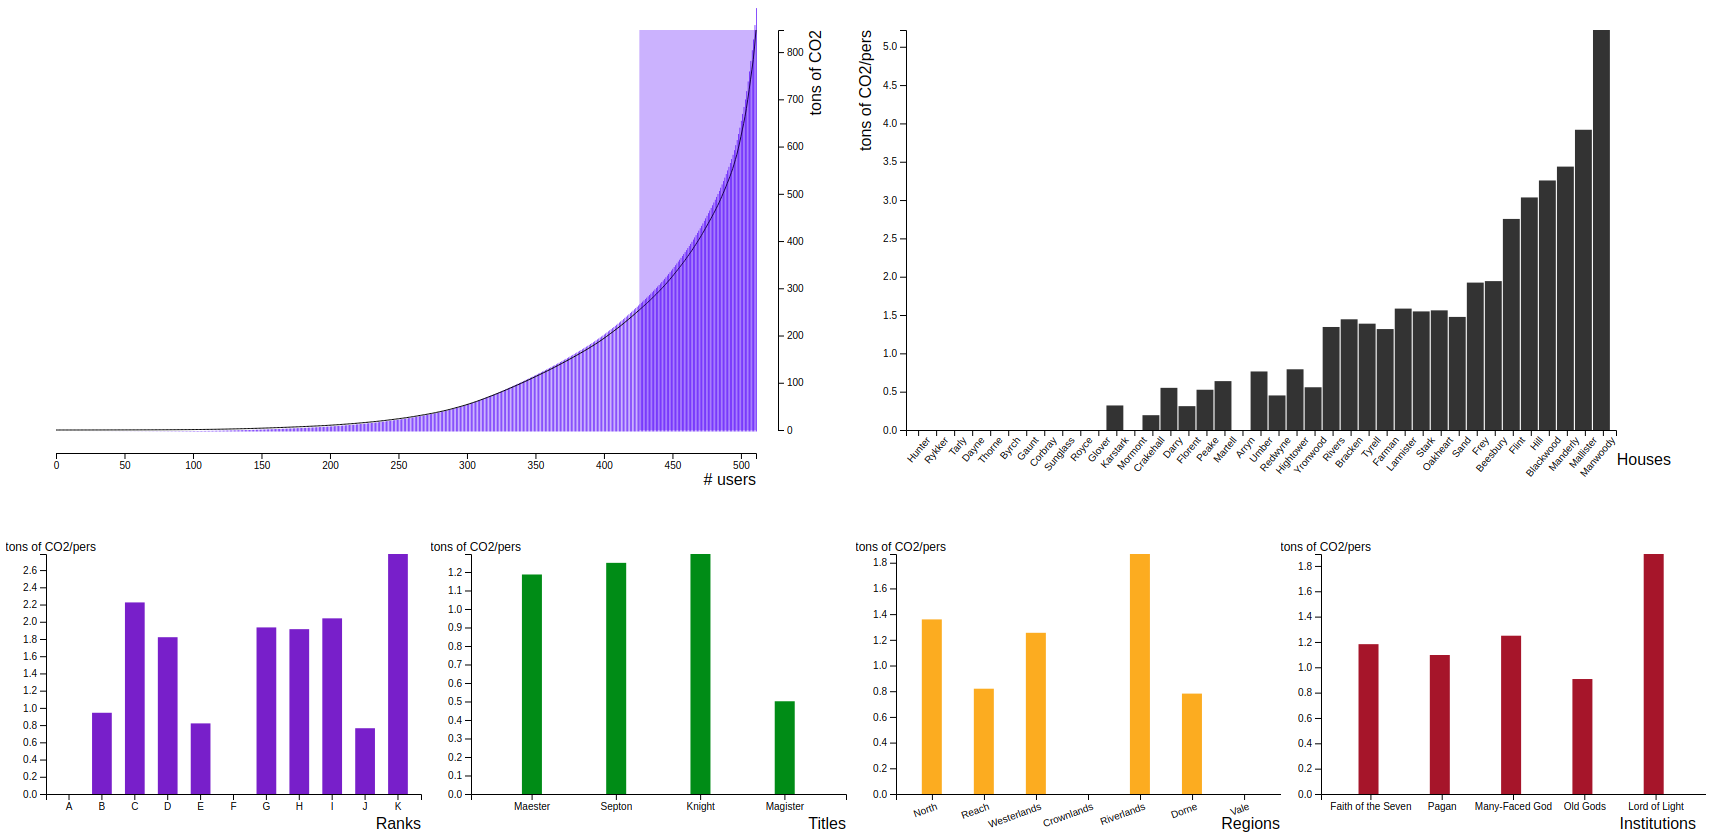
\includegraphics[scale=0.28]{img/ceo2_last.png}
	\caption{CO${_2}$ - subsets statistics. Last 1/6 of users selected}
	\label{fig:ceo2_last}
\end{figure}
Now we want to get even more detailed information about subgroups of users that emit similar amounts of CO$_2$. For example, in Figure \ref{fig:ceo2_last}, I selected the last 1/6 of users: many of them live in Manwoody house or have the title K. On the other hand, we do not encounter them in Vale or Crownlands regions and do not have the titles A and F. 

Let's take a look to the first 1/6 of users selected(Figure \ref{fig:ceo2_first}). The intuitions that many of them are part of the houses that pollute the least(from Figure \ref{fig:vis_1}) or that they normally have the title A are now confirmed. It is interesting that they also are part of the Lord of Light Institution, the one in which we find the 1/6 of users that pollute the most.

In conclusion, I think this visualization gives a good intuition about the CO$_2$ distribution over the subsets of users. Even though my way of "brushing" the data is not as versatile as a normal slider, it still offers interesting details about the predominant characteristics of some representative subgroups of users.
 

\begin{figure}[H]
	\centering
	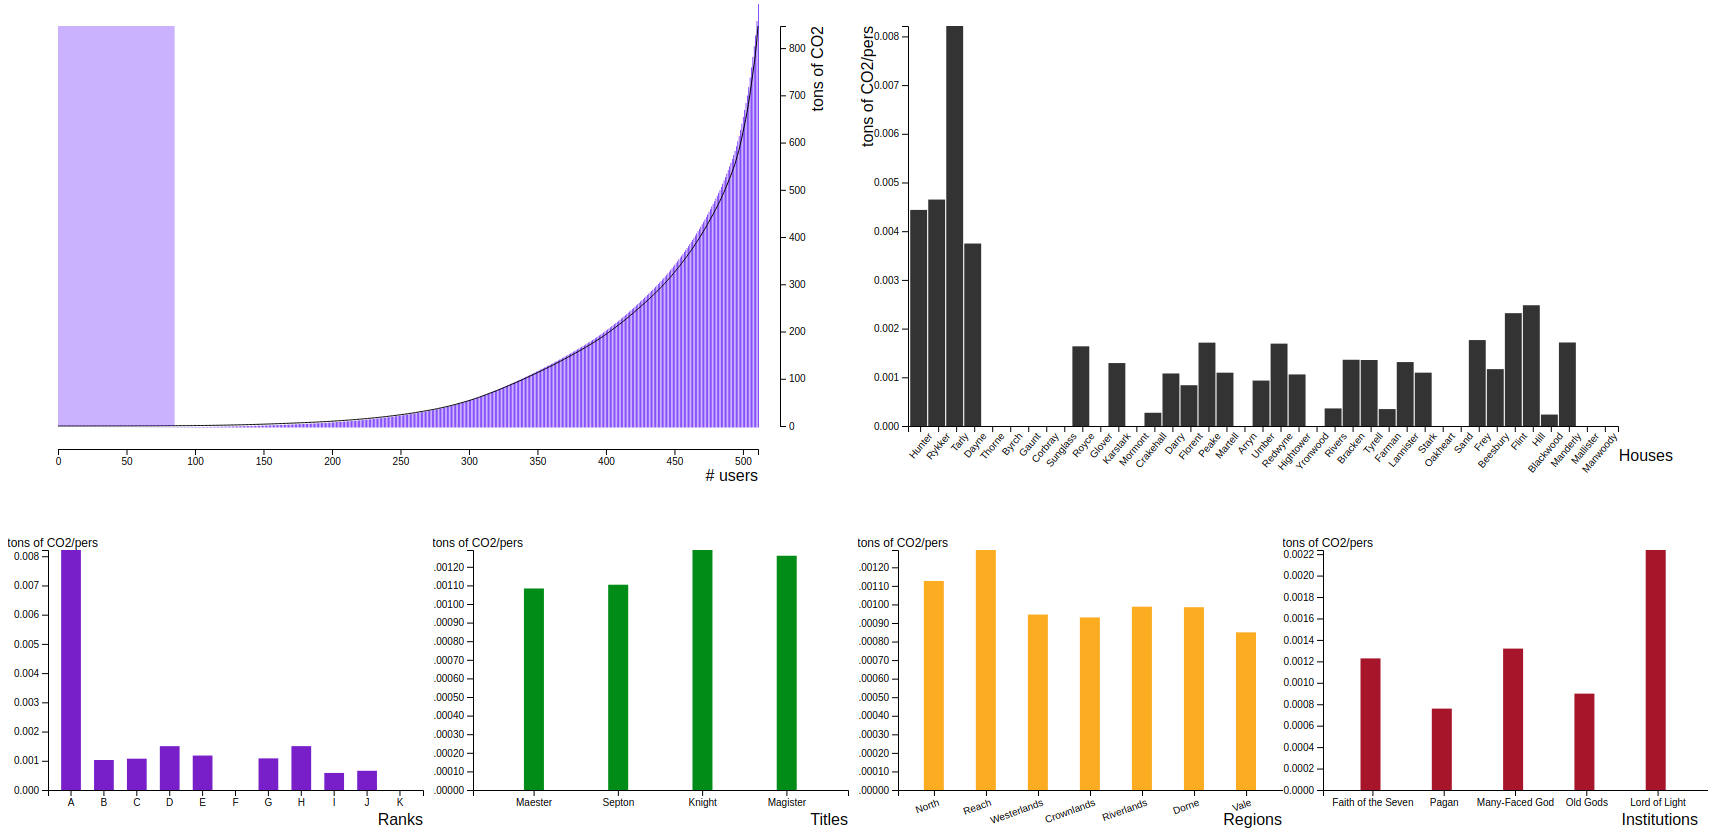
\includegraphics[scale=0.28]{img/ceo2_first.png}
	\caption{CO${_2}$ - subsets statistics. First 1/6 of users selected}
	\label{fig:ceo2_first}
\end{figure}




\newpage

\bibliographystyle{plain}
\bibliography{bibliography}


\end{document}
